%%%%%%%%%%%%%%%%%%%%%%%VICARIOUS%%%%%%%%%%%%%%%%%%%%%%%%%%%%%%%%%%%%%%%
% 																	%
% Template for presentation in Latex`s Beamer Class					%
% Using the default Berlin theme, can be replaced by other themes		%
% logo in the upper right can be replaced by new .png, gif, eps etc	%
% 																	%
%%%%%%%%%%%%%%%%%%%%%%%%%%%%%%%%%%%%%%%%%%%%%%%%%%%%%%%%%%%%%%%%%%%%%%%
\documentclass[xcolor=dvipsnames, aspectratio=169]{beamer}
\usetheme{Berlin}
\usecolortheme[named=LimeGreen]{structure}
\usepackage{beamerthemesplit} % kam neu dazu
\usepackage[ngerman]	{babel}			
\usepackage{t1enc}						
\usepackage[utf8]{inputenc}			
\usepackage{amsmath}
\usepackage{graphicx}
\graphicspath{{pictures/}}
\usepackage{amssymb}
\usepackage{amsfonts}
\usepackage{caption}
\usepackage{multimedia}
\usepackage{tikz}
\usepackage{listings}
\usepackage{acronym}
\usepackage{subfig}

\usepackage{lmodern}
\usepackage{multicol}

\definecolor{pblue}{rgb}{0.13,0.13,1}
\definecolor{pgreen}{rgb}{0,0.5,0}
\definecolor{pred}{rgb}{0.9,0,0}
\definecolor{pgrey}{rgb}{0.46,0.45,0.48}

\lstset{
    escapeinside={(*}{*)}
}

\lstdefinestyle{Java}{
  showspaces=false,
  showtabs=false,
  tabsize=2,
  breaklines=true,
  showstringspaces=false,
  breakatwhitespace=true,
  commentstyle=\color{pgreen},
  keywordstyle=\color{pblue},
  stringstyle=\color{pred},
  basicstyle=\footnotesize\ttfamily,
  numbers=left,
  numberstyle=\tiny\color{gray}\ttfamily,
  numbersep=7pt,
  %moredelim=[il][\textcolor{pgrey}]{$$},
  moredelim=[is][\textcolor{pgrey}]{\%\%}{\%\%},
  captionpos=b
}

\lstdefinestyle{basic}{  
  basicstyle=\footnotesize\ttfamily,
  breaklines=true
  numbers=left,
  numberstyle=\tiny\color{gray}\ttfamily,
  numbersep=7pt,
  backgroundcolor=\color{white},
  showspaces=false,
  showstringspaces=false,
  showtabs=false,
  frame=single,
  rulecolor=\color{black},
  captionpos=b,
  keywordstyle=\color{blue}\bf,
  commentstyle=\color{gray},
  stringstyle=\color{green},
  keywordstyle={[2]\color{red}\bf},
}


\lstdefinelanguage{custom}
{
morekeywords={public, void},
sensitive=false,
morecomment=[l]{//},
morecomment=[s]{/*}{*/},
morestring=[b]",
}


\lstdefinestyle{BashInputStyle}{
  language=bash,
  showstringspaces=false,
  basicstyle=\small\sffamily,
  numbers=left,
  numberstyle=\tiny,
  numbersep=5pt,
  frame=trlb,
  columns=fullflexible,
  backgroundcolor=\color{gray!20},
  linewidth=0.9\linewidth,
  xleftmargin=0.1\linewidth
}

%Logo in the upper right just change if you know what you are doing^^
\addtobeamertemplate{frametitle}{}{%
\begin{tikzpicture}[remember picture,overlay]
\node[anchor=north east,yshift=2pt] at (current page.north east) {
\includegraphics[height=1.8cm]{htw}};
\end{tikzpicture}}

\begin{document}
\bibliographystyle{alpha}
\title{Netzwerke -- Übung WiSe2018/19}
\subtitle{Backbone Routing\\
		\href{mailto:Benjamin.Troester@HTW-Berlin.de}{Benjamin.Troester@HTW-Berlin.de}\\
		PGP: ADE1 3997 3D5D B25D 3F8F 0A51 A03A 3A24 978D D673 }
\author{Benjamin Tröster}

\date{}

\begin{frame}
\titlepage

\end{frame}

\section*{Road-Map}
\begin{frame}
\frametitle{Road-Map}
\begin{multicols}{2}
  \tableofcontents
\end{multicols}
\end{frame}

\section{Aktueller Stand}
\begin{frame}
	\frametitle{Aktueller Stand}
	\begin{itemize}
		\item Zwei LANs verbunden durch Router
		\item Router als Zwischenknoten in beiden Netzwerken durch eigene IP-Adresse vertreten
		\item Kommunikation außerhalb dieser beiden Netzwerke (noch) nicht möglich
		\begin{itemize}
			\item \textbf{Hinweis:} Es wäre aber durch möglich gewesen!
		\end{itemize}
	\end{itemize}
\end{frame}

\section{Backbone}
\begin{frame}
	\frametitle{Backbone Routing}
	 \begin{tabular}{lc}
 \hspace*{-1.3cm} 
 \parbox{0.65\linewidth}{
	\begin{itemize}
		\item Nächster Schritt: Jede Tischreihe bekommt einen zusätzlichen Router
		\item $\rightarrow$ Backbone-Router: kennt Routen zu allen andern Netzwerken
		\begin{itemize}
			\item Rechnernetze können miteinander kommunizieren
		\end{itemize}
	\end{itemize} } 
& \begin{tabular}{l}
 \begin{tabular}{c}
           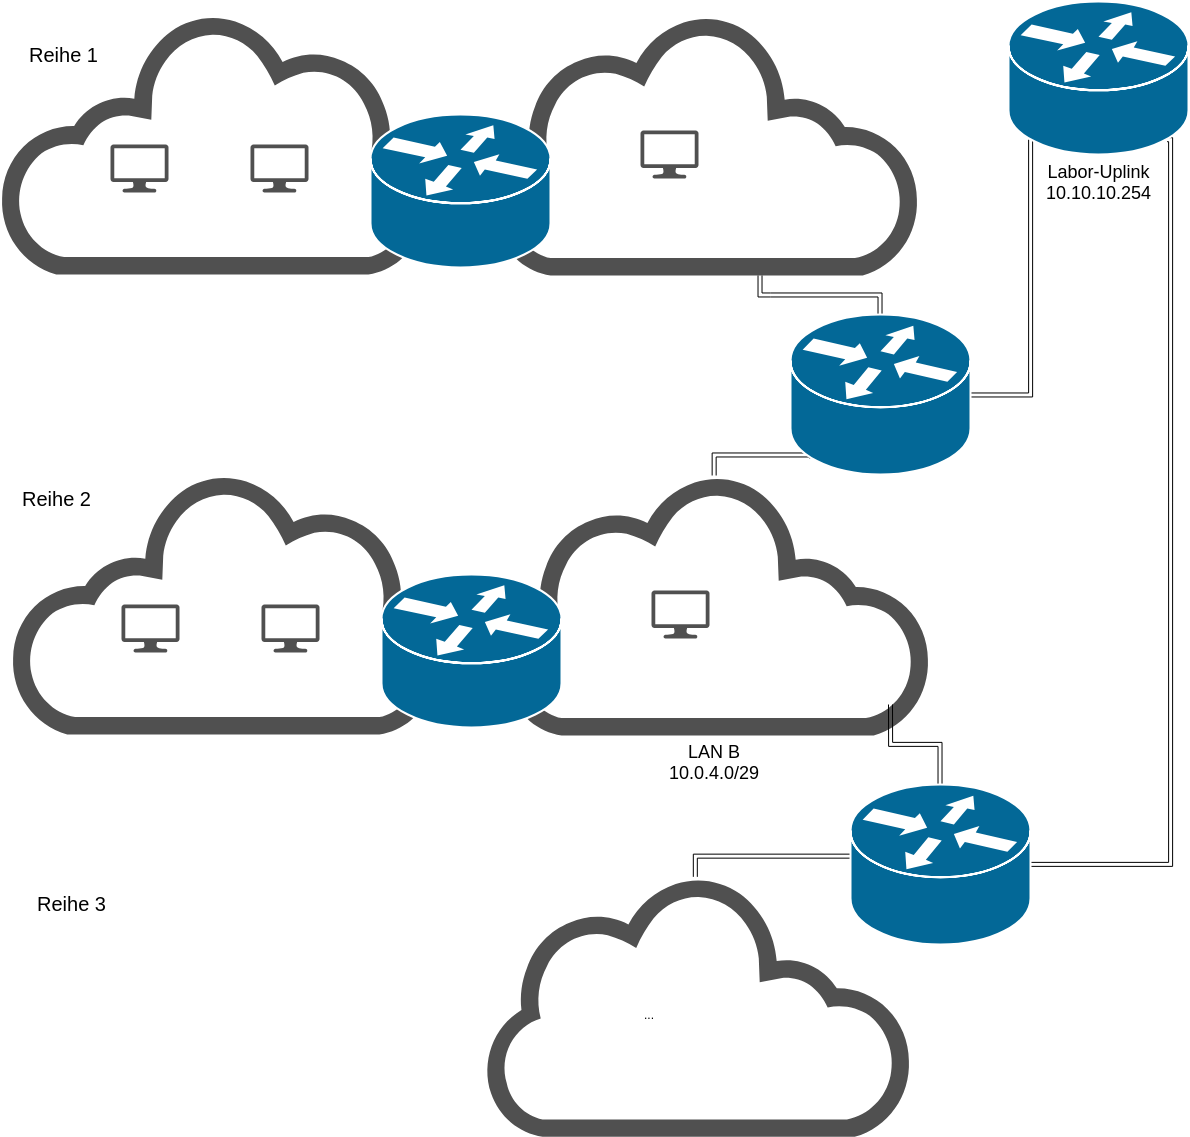
\includegraphics[scale=0.125]{backbone}
           \end{tabular}
\end{tabular}\\
\end{tabular}
\end{frame}

\section{Uplink}
\begin{frame}
\frametitle{Uplink}
	\begin{itemize}
		\item Ihr Backbone-Router ist zusätzlich zuständig für den Uplink
		\begin{itemize}
			\item D.h. dieser Rechner verbindet Sie ins DFN/Internet
		\end{itemize}
		\item Der Labor-Router ist in diesem Fall ihr Default-Gateway
		\begin{itemize}
			\item IPv4: 10.10.10.254
		\end{itemize}
		\item Alle Pakete, die nicht direkt an andere Raspberry Pis adressiert sind werden über das Default-Gateway geschickt
		\item D.h. Default-Gateway nimmt alle nicht adressierbaren Pakete entgegen und muss sich darum kümmern
		\item Uplink besitzt zudem einen DNS-Server um Domainnamen in IP-Adressen und andersherum zu übersetzen
		\item Ebenso findet hier die Übersetzung der privaten Adressen in \textbf{eine} öffentliche Adresse statt -- SNAT via \emph{iptables}
	\end{itemize}
\end{frame}

\section{iptables}
\begin{frame}
\frametitle{Firewalls}
	\begin{itemize}
		\item Firewall: Network-Security-System das eingehenden \& ausgehenden Netzwerkverkehr überwacht
		\item Analysiert Verkehr anhand von festgelegten Regeln -- wie wird mit dem Netzwerkverkehr umgegangen
		\item Stellt in vielen Netzwerken Barriere dar, um vertrauenswürdige von nicht vertrauenswürdigen Netzen zu trennen
	\end{itemize}
\end{frame}

\begin{frame}
\frametitle{iptables}
	\begin{itemize}
		\item \emph{iptables}: Kommandozeilen-Tool für Konfiguration der Tabellen im Kernel
		\item Tables im wesentlichen Reihen von Netfilter-Modulen (sog. \emph{chains} und \emph{rules})
		\item \emph{iptables} wird oftmals als Firewall genutzt
		\begin{itemize}
			\item Kann durch entsprechend Tabelleneinträge Netzwerkverkehr filtern, weiterleiten etc.
		\end{itemize}
		\item \emph{iptables} ist auf \emph{IPv4} beschränkt
		\begin{itemize}
			\item Entsprechend: \emph{ip6tables}, \emph{arptables}
		\end{itemize}
	\end{itemize}
\end{frame}

\section{NAT}
\begin{frame}
\frametitle{Network-Address-Translation -- NAT}
\vspace*{-0.5cm}
	\begin{itemize}
		\item Im Labor nutzen Sie nur private IP-Adressen -- im Internet benötigen Sie jedoch eine öffentliche IP-Adresse
		\item Aufgrund des Adressmangels unter \emph{IPv4}, dynamische Vergabe von IPv4-Adressen durch den ISP
		\item In vielen Netzwerken sind die Geräte daher nur mit privaten Adressen erreichbar
		\item Durch NAT kann eine Auflösung von öffentlicher auf privater IP-Adresse vorgenommen
		\begin{itemize}
			\item NAT-Router übersetzt lokale, private \emph{IPv4}-Adressen in öffentliche Adresse
			\item Zuordnung aufgrund von NAT-Tabellen -- D.h. es wird ein NAT-Port einer IP-Adresse samt dessen Port zugeordnet
			\item NAT-Router muss für jedes eingehende Paket eine Übersetzung vornehmen
		\end{itemize}
		\item Übersetzung von lokaler \emph{IPv4}-Adresse auf öffentliche via \emph{iptables}
	\end{itemize}
\end{frame}

\section{DNS}
\begin{frame}
	\frametitle{Domain Name System -- DNS}
	\begin{itemize}
		\item DNS sorgt für das Mapping von Domainname auf IP-Adresse
		\begin{itemize}
			\item \glqq Nur\grqq\ kosmetisch notwendig, da Menschen i.d.R. Namen besser memorieren als Zahlen
		\end{itemize}
		\item DNS ist selbst eine verteilte Datenbank
		\item Sorgt durch Look-Ups (iterativ/iterativ) für Übersetzung
		\item Später mehr dazu...
	\end{itemize}
\end{frame}

\section{IPv6}
\begin{frame}
	\frametitle{IPv6}
	\begin{itemize}
		\item 
	\end{itemize}
\end{frame}

\section{Tools}
\begin{frame}
	\frametitle{Tools}
	\begin{itemize}
		\item \emph{iproute2}: \emph{ip addr}, \emph{ip route}, \emph{ip link} 
		\item \emph{net-tools}: \emph{ifconfig}, \emph{route}, \emph{netstat}
		\item \emph{nc}
		\item \emph{iptables}
	\end{itemize}
\end{frame}
\end{document}